\chapter{Sample Title}

Lorem ipsum dolor sit amet, consectetur adipiscing elit, sed do eiusmod tempor incididunt ut labore et dolore magna aliqua. Ut enim ad minim veniam, quis nostrud exercitation ullamco laboris nisi ut aliquip ex ea commodo consequat. Duis aute irure dolor in reprehenderit in voluptate velit esse cillum dolore eu fugiat nulla pariatur. Excepteur sint occaecat cupidatat non proident, sunt in culpa qui officia deserunt mollit anim id est laborum.

\section{Example section.} {
This is an example section.

\subsection{Referencing} { \label{referencing}
In this subsection we cite \cite{Einstein}.

We also refer to this section as \ref{referencing}.

And we refer to the appendix containing the code as appendix \ref{code}.

We can refer to the figure we made like this: figure \ref{nrctypes}.
}

\subsection{Including code} {
In this subsection we include the following code snippet:

\begin{lstlisting}
//comment
implicit def IntRing: Ring[Int] = new Ring[Int] {
  def add(t1: Int, t2: Int): Int = t1 + t2
  def negate(t1: Int): Int = -t1
}
\end{lstlisting}

We also include this inline reference to \lstinline{trait Ring[T]}.
}

\subsection{Calculus} {
In this subsection we show how we write the symbols for the calculus:
 
\[ \R := \prim{Int} \:|\: \R \times  \R \: | \: \coll{\K}{\R} \]

\[ \K := \prim{Dom} \OR  [\R]  \OR \prim{Label} \]

\[ \Bag{\K} \]

\[ (\R,0_\R,+_\R,-_\R,1_\R,*_\R) \]

\[ \langle \mathit{k}_1, k_2 \rangle \: k.\_ i \: r_1 \cdot r_2 \{ x => r \} \]

\[ \ForIf{x}{X}{p(x)} \YieldP{k}{r} \]

\[ \delta_X(r) \]

\[ (\cdot)^F  \: (\cdot)^\Gamma \: \odot \]
}

\subsection{Figures} {

\pgfplotsset{
        % use this `compat' level or higher to use the feature of specifying
        % `bar width' in axis units
        compat=1.7,
    }
    \pgfplotstableread[row sep=\\,col sep=&]{
        no-batches & regular  & shred-inc  & shred-acc \\%   & carG    \\
        5    & 52.1 & 20.9 & 22.2   \\%& 100000  \\
        10      & 84.1 & 29.9 & 34.9  \\%& 100000  \\
        25 & 196 & 53.1 & 55.0 \\%& 1000000 \\
    }\QOne
    
     \pgfplotstableread[row sep=\\,col sep=&]{
        no-batches & regular  & shred-inc  & shred-acc \\%   & carG    \\
        5    & 57.4 & 70.3 & 71.5   \\%& 100000  \\
        10      & 103 & 118 & 121  \\%& 100000  \\
        25 & 246 & 257 & 270 \\%& 1000000 \\
    }\QTwo
    
    \pgfplotstableread[row sep=\\,col sep=&]{
        no-batches & regular  & shred-inc  & shred-acc \\%   & carG    \\
        5    & 107 & 83.0 & 83.8   \\%& 100000  \\
        10      & 189 & 131 & 135  \\%& 100000  \\
        25 & 431 & 282 & 289 \\%& 1000000 \\
    }\QThree
    
     \pgfplotstableread[row sep=\\,col sep=&]{
        no-batches & regular  & shred-inc  & shred-acc \\%   & carG    \\
        5    & 3.06 & 2.12 & 2.61   \\%& 100000  \\
        10      & 5.76 & 3.66 & 5.18  \\%& 100000  \\
        25 & 14.1 & 10.2 & 13.6 \\%& 1000000 \\
    }\QFour
    
In this subsection we show how to make figures from our equations.


\begin{figure}
\begin{tabular}{cc}

\begin{tikzpicture}
\begin{axis}[
    title=Q1,
     width=0.5\textwidth,
    height=.5\textwidth,
    ymin=0,
    %yticklabel style={/pgf/number format/fixed},
    ymajorticks=false,
    ylabel={Time taken (seconds)},
    xlabel={Number of batches},
    xtick=data,
    xticklabels from table={\QOne}{no-batches},
    bar width=0.2,
    ybar=2pt,
    enlarge x limits={abs=0.55},
    nodes near coords,
    nodes near coords style={font=\tiny},
    legend pos=north west,
    legend style={legend columns=1},
]
    \addplot table [x expr=\coordindex,y=regular]{\QOne};
    \addplot table [x expr=\coordindex,y=shred-inc]{\QOne};
    \addplot table [x expr=\coordindex,y=shred-acc]{\QOne};
    %\addplot table [x expr=\coordindex,y=carG]{\mydata};

    \legend{regular, shred-inc, shred-acc}
\end{axis}
\end{tikzpicture}
& \begin{tikzpicture}
\begin{axis}[
    title=Q2,
     width=0.5\textwidth,
    height=.5\textwidth,
    ymin=0,
    %yticklabel style={/pgf/number format/fixed},
    ymajorticks=false,
    ylabel={Time taken (seconds)},
    xlabel={Number of batches},
    xtick=data,
    xticklabels from table={\QTwo}{no-batches},
    bar width=0.2,
    ybar=2pt,
    enlarge x limits={abs=0.55},
    nodes near coords,
    nodes near coords style={font=\tiny},
    legend pos=north west,
    legend style={legend columns=-1},
]
    \addplot table [x expr=\coordindex,y=regular]{\QTwo};
    \addplot table [x expr=\coordindex,y=shred-inc]{\QTwo};
    \addplot table [x expr=\coordindex,y=shred-acc]{\QTwo};
    %\addplot table [x expr=\coordindex,y=carG]{\mydata};

    %\legend{regular, shred-inc, shred-acc}
\end{axis}
\end{tikzpicture}

\\ \\ \\

\begin{tikzpicture}
\begin{axis}[
    title=Q3,
     width=0.5\textwidth,
    height=.5\textwidth,
    ymin=0,
    %yticklabel style={/pgf/number format/fixed},
    ymajorticks=false,
    ylabel={Time taken (seconds)},
    xlabel={Number of batches},
    xtick=data,
    xticklabels from table={\QThree}{no-batches},
    bar width=0.2,
    ybar=2pt,
    enlarge x limits={abs=0.55},
    nodes near coords,
    nodes near coords style={font=\tiny},
    legend pos=north west,
    legend style={legend columns=-1},
]
    \addplot table [x expr=\coordindex,y=regular]{\QThree};
    \addplot table [x expr=\coordindex,y=shred-inc]{\QThree};
    \addplot table [x expr=\coordindex,y=shred-acc]{\QThree};
    %\addplot table [x expr=\coordindex,y=carG]{\mydata};

    %\legend{regular, shred-inc, shred-acc}
\end{axis}
\end{tikzpicture}
& \begin{tikzpicture}
\begin{axis}[
    title=Q4,
     width=0.5\textwidth,
    height=.5\textwidth,
    ymin=0,
    %yticklabel style={/pgf/number format/fixed},
    ymajorticks=false,
    ylabel={Time taken (seconds)},
    xlabel={Number of batches},
    xtick=data,
    xticklabels from table={\QFour}{no-batches},
    bar width=0.2,
    ybar=2pt,
    enlarge x limits={abs=0.55},
    nodes near coords,
    nodes near coords style={font=\tiny},
    legend pos=north west,
    legend style={legend columns=-1},
]
    \addplot table [x expr=\coordindex,y=regular]{\QFour};
    \addplot table [x expr=\coordindex,y=shred-inc]{\QFour};
    \addplot table [x expr=\coordindex,y=shred-acc]{\QFour};
    %\addplot table [x expr=\coordindex,y=carG]{\mydata};

   % \legend{regular, shred-inc, shred-acc}
\end{axis}
\end{tikzpicture}
\end{tabular}
\end{figure}








\begin{figure}
\begin{equation*}
\begin{aligned}[c]
\R := \prim{Int} \:|\: \R \times  \R \: | \: \coll{\K}{\R} \\
\R := \prim{Int} \:|\: \R \times  \R \: | \: \coll{\K}{\R}
\end{aligned}
\qquad
\begin{aligned}[c]
\K := \prim{Dom} \OR  [\R]  \OR \prim{Label} \\
\K := \prim{Dom} \OR  [\R]  \OR \prim{Label}
\end{aligned}
\end{equation*}
\caption{The type system of the NRC}
\label{nrctypes}
\end{figure}










\begin{figure}
\centering
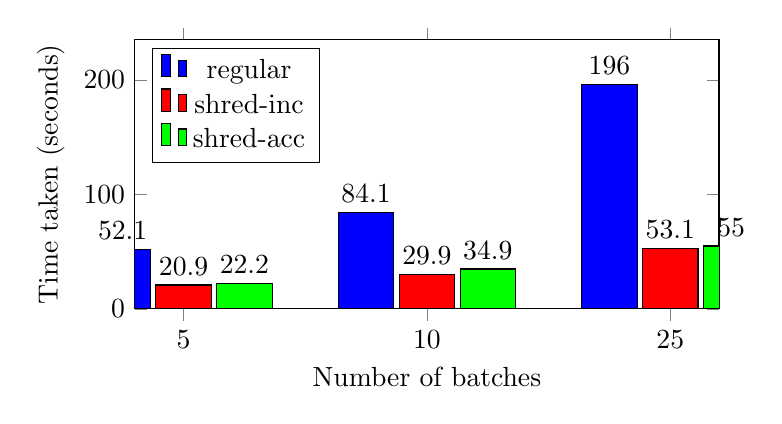
\begin{tikzpicture}
    \begin{axis}[
        ybar,
        ymin=0,
        width  = 9cm,
        height = 5cm,
        bar width=20pt,
        ylabel={Time taken (seconds)},
        xlabel={Number of batches},
        nodes near coords,
 %      nodes near coords align=below, % places labels inside bars
        symbolic x coords={5,10,25},
        xtick = data,
        xtick align=outside,
       enlarge y limits={value=0.2,upper},
        %enlarge x limits={value=0},
        legend pos=north west
    ]
    \addplot[fill=blue] coordinates {(5, 52.1) (10, 84.1) (25, 196)};
    \addplot[fill=red] coordinates {(5, 20.9) (10, 29.9) (25, 53.1)};
    \addplot[fill=green] coordinates {(5, 22.2) (10, 34.9) (25, 55)};
      \legend{regular, shred-inc, shred-acc}
    \end{axis}
\end{tikzpicture}
\end{figure}
}
	

